\section{Polynomial Hierarchy}
\begin{figure}[h]
    \centering
    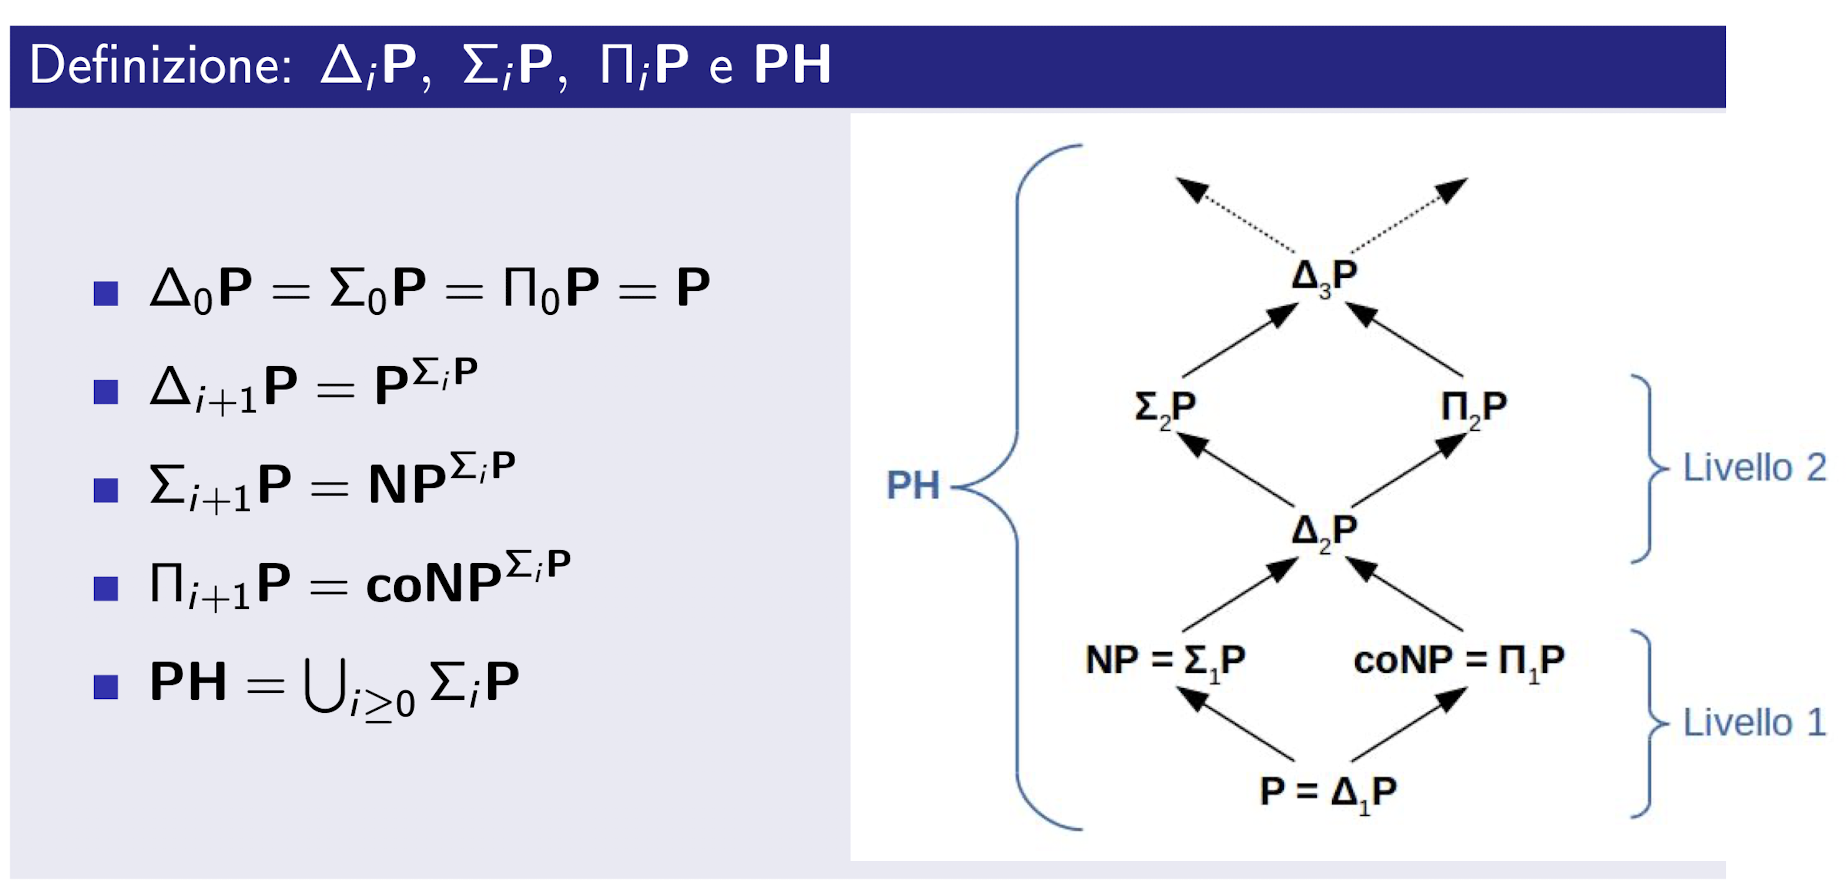
\includegraphics[width=1\textwidth]{img/ph.png}
    \caption{Polynomial Hierarchy}
\end{figure}
Since $\Sigma_0\mathbf{P} = \mathbf{P}$ does not help polynomial-time oracle machines, the first level of this hierarchy makes up our familiar important complexity classes: 
\[
\Delta_1\mathbf{P} = \mathbf{P}, \quad \Sigma_1\mathbf{P} = \mathbf{NP}, \quad \Pi_1\mathbf{P} = \mathbf{coNP}.
\]
The second level starts with the class $\Delta_2\mathbf{P} = \mathbf{P}^{\mathbf{NP}}$ studied in the previous section, and continues with $\Sigma_2\mathbf{P} = \mathbf{NP}^{\mathbf{NP}}$, and its complement $\Pi_2\mathbf{P} = \mathbf{coNP}^{\mathbf{NP}}$. As with the first level, there is every reason to believe that all three classes are distinct. The same holds for the third level, and so on. Naturally, the three classes at each level are related by the same inclusions that we know about $\mathbf{P}$, $\mathbf{NP}$, and $\mathbf{coNP}$. Also, each class at each level includes all classes at previous levels.
\begin{defbox}[Theorem 17.8]
Let $L$ be a language, and $i \geq 1$. $L \in \Sigma_i\mathbf{P}$ if and only if there is a polynomially balanced relation $R$ such that the language $\{x; y : (x, y) \in R\}$ is in $\Pi_{i-1}\mathbf{P}$ and
\[
L = \{ x : \text{there is a } y \text{ such that } (x, y) \in R \}
\]
\end{defbox}
\begin{proof}
    omitted
\end{proof}
\begin{defbox}[Corollary 1]
Let $L$ be a language, and $i \geq 1$. $L \in \Pi_i\mathbf{P}$ if and only if there is a polynomially balanced binary $R$ such that the language $\{x; y : (x, y) \in R\}$ is in $\Sigma_{i-1}\mathbf{P}$ and
\[
L = \left\{ x : \text{ for all } y \text{ with } |y| \leq |x|^k,\, (x, y) \in R \right\}.
\]
\end{defbox}
\begin{proof}
Just recall that $\Pi_i\mathbf{P}$ is precisely $\mathbf{co}\Sigma_i\mathbf{P}$.
\end{proof}
Notice that in the description of $L$ in Corollary 1 we must explicitly state for the universally quantified string $y$ the bound $|y| \leq |x|^k$. Since $R$ is known to be polynomially balanced, this constraint is, in this context, superfluous, and will be omitted. Also, we shall use quantifiers such as $\forall x$ and $\exists y$ in the descriptions of languages such as the one displayed in Corollary 2 below. This will help bring out the elegant mathematical structure of these descriptions, as well as their affinity with logic.

\medskip

In order to get rid of the recursion in the previous Theorem, let us call a relation $R \subseteq (\Sigma^*)^{i+1}$ polynomially balanced if, whenever $(x, y_1, \ldots, y_i) \in R$, we have that $|y_1|, \ldots, |y_i| \leq |x|^k$ for some $k$.
\begin{defbox}[Corollary 2]
Let $L$ be a language, and $i \geq 1$. $L \in \Sigma_i\mathbf{P}$ if and only if there is a polynomially balanced, polynomial-time decidable $(i+1)$-ary relation $R$ such that
\[
L = \left\{ x : \exists y_1 \forall y_2 \exists y_3 \cdots Q y_i \text{ such that } (x, y_1, \ldots, y_i) \in R \right\}
\]
where the $i$th quantifier $Q$ is ``for all'' if $i$ is even, and ``there is'' if $i$ is odd.
\end{defbox}
\begin{proof}
    Repeatedly replace languages in $\Pi_j\mathbf{P}$ or $\Sigma_j\mathbf{P}$ by their certificate forms as in Theorem and its Corollary 1.
\end{proof}
Using these characterizations we can prove the basic fact concerning the polynomial hierarchy: As it is built by patiently adding layer after layer, always using the previous layer as an oracle for defining the next, the resulting structure is extremely fragile and delicate. Any jitter, at any level, has disastrous consequences further up:

\begin{defbox}[Theorem 17.9]
If for some $i \geq 1$ $\Sigma_i\mathbf{P} = \Pi_i\mathbf{P}$, then for all $j > i$ $\Sigma_j\mathbf{P} = \Pi_j\mathbf{P} = \Delta_j\mathbf{P} = \Sigma_i\mathbf{P}$.
\end{defbox}

\begin{proof}
It suffices to show that $\Sigma_i\mathbf{P} = \Pi_i\mathbf{P}$ implies $\Sigma_{i+1}\mathbf{P} = \Sigma_i\mathbf{P}$. So, consider a language $L \in \Sigma_{i+1}\mathbf{P}$. By Theorem 17.8 there is a relation $R$ in $\Pi_i\mathbf{P}$ with 
\[
L = \{x : \text{there is a } y \text{ such that } (x, y) \in R\}.
\]
But since $\Pi_i\mathbf{P} = \Sigma_i\mathbf{P}$, $R$ is in $\Sigma_i\mathbf{P}$. That is, $(x, y) \in R$ if and only if there is a $z$ such that $(x, y, z) \in S$ for some relation $S \in \Pi_{i-1}\mathbf{P}$. Thus $x \in L$ if and only if there is a string $y, z$ such that $(x, y, z) \in S$, where $S \in \Pi_{i-1}\mathbf{P}$. But this means that $L \in \Sigma_i\mathbf{P}$.
\end{proof}

The statements of many results in complexity theory end like that of Theorem 17.9: ``then for all $j > i$ $\Sigma_j\mathbf{P} = \Pi_j\mathbf{P} = \Delta_j\mathbf{P} = \Sigma_i\mathbf{P}$.'' This conclusion is usually abbreviated ``then the polynomial hierarchy collapses to the $i$th level.'' For example:

\begin{defbox}[Corollary]
If $\mathbf{P} = \mathbf{NP}$, or even if $\mathbf{NP} = \mathbf{coNP}$, the polynomial hierarchy collapses to the first level.
\end{defbox}
The last corollary makes one thing abundantly clear: In the absence of a proof that $\mathbf{P} \neq \mathbf{NP}$, there is no hope of proving that the polynomial ``hierarchy'' is indeed a hierarchy of classes each properly containing the next (although, once again, we strongly believe that it is).
The non-monotonic logics were introduced in AI to allow reasoning with incomplete information. The idea is to make plausible assumption that could end up being false in the future. Some examples of non-monotonic logics are Circumscription, Default logic and Answer Set Programming (ASP). The reasoning in the proposition versione of these logics is positioned at the 2° level of the polynomial hierarchy. 